\section{Estructuras} \label{sec:estructuras}

Además, de los objetos mencionados, agregamos 3 estructuras adicionales para facilitar el
renderizado de objetos más complejos:

\begin{itemize}
    \item Lista de objetos
    \item Malla de triángulos
    \item KD Tree
\end{itemize}

A continuación explicamos brevemente la implementación de cada uno.
\subsection{Lista de objetos} \label{subsec:lista_objetos}

Tiene una implementación muy directa, ya que como su nombre indica, solo almacena una lista
de objetos (básicos u otras estructuras).
La colisión de un rayo contra este se calcula como el punto más cercano de colisión entre el rayo y
alguno de los objetos que almacena, si es que hubiese colisión.

Es una estructura de utilidad para facilitar el renderizado de escenas o para crear otras
estructuras más complejas, como las que veremos a continuación.

\subsection{Malla de Triángulos} \label{subsec:malla_triangulos}

Las mallas de triángulos por lo general consisten de miles de objetos, por lo que la
implementación de esta estructura toma como parámetro un archivo en el que se definen los mismos.
El archivo consiste de lineas de tipo vértice, en el que se indican las coordenadas de cada
vértice, y de tipo cara, en el que se indican que vertices componen a cada triangulo.
Dejando de lado esa diferencia, la implementación es prácticamente la misma que la lista de objetos,
solo que almacena triángulos.

En la figura~\ref{fig:escena_malla_pato} podemos ver el render del modelo de un pato.

\begin{figure}[H]
    \centering
    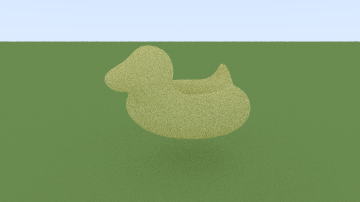
\includegraphics[width=.9\textwidth]{imgs/escena_malla_pato}
    \caption{Render de una malla de triángulos.}
    \label{fig:escena_malla_pato}
\end{figure}

Sin embargo, debido a la sencillez de la implementación de la lista de objetos, esta estructura
resulta muy lenta ya que se debe recorrer los miles de triángulos uno por uno para detectar
colisiones.
Para poder mitigar el tiempo de procesamiento, utilizamos la siguiente estructura para calcular
menos colisiones, el KD Tree.

\subsection{KD Tree} \label{subsec:kd_tree}

El problema que tiene la implementación anterior es que la complejidad para saber si un rayo
colisiona con algún triángulo de la malla crece con la cantidad de objetos en la lista.

Los \textit{axis-aligned bounding boxes} (AABB) son estructuras que mejoran la complejidad
dependiendo del tipo (Octree, BPS Tree, KD Tree, etc.).
Logran esto dividiendo el espacio en partes iguales, y encerrando cada parte en una caja que
contenga todos sus objetos.
Luego cada partición del espacio se divide de la misma forma, creando así una jerarquía de cajas
asociada a cada nodo de un árbol.
La raíz del árbol representa la caja más grande que contiene todos los objetos, y los nodos hijos
están asociados a cada partición del espacio, con sus respectivas cajas.

El \textit{KD Tree} es una estructura AABB en el que en cada paso de la división del espacio, se
hace un único corte en el eje donde la longitud de la caja es mayor.
Esto significa que el árbol resultante es un árbol binario, ya que cada espacio se divide en 2.

Esta nueva estructura puede recibe como parámetro una lista de objetos y un entero indicando
cuantos elementos debe tener las hojas del árbol.
Luego se procede a dividir el espacio hasta llegar a nodos que contengan como máximo la cantidad
indicada.
De esta forma, si se especifica como lista de objetos una malla de 16000 triángulos y como cantidad
máxima 500 objetos, el espacio se divide hasta llegar a un árbol de altura 6 con 32 hojas, cada una
con 500 triángulos.

Esta estructura nos permitió acelerar el renderizado tanto de las mallas de triángulos, como de
escenas complejas que cuentan con muchos objetos.